\documentclass[12pt]{article} 
\usepackage[x11names]{xcolor}
\usepackage{setspace}  %line spacing
\usepackage{parskip}    %spaced paragraphs
\usepackage{tabularx}
\usepackage{subcaption}
\usepackage{float}
\usepackage{afterpage}
\usepackage[hidelinks]{hyperref}

\usepackage{pgfplots}
\pgfplotsset{compat=1.18}

% \usepackage{fourier-otf}    % font pack
% \usepackage{helvet}
\renewcommand{\familydefault}{\sfdefault}
% \usepackage[T1]{fontenc}
\usepackage{sansmath}
\sansmath

\usepackage{amsmath}    
\addtolength{\jot}{0.5em} % spacing for align environments

\usepackage{fancyhdr}
\setlength{\headheight}{15pt}

\usepackage{geometry}   %set margins
\geometry{a4paper, margin=1.5cm}

\usepackage{graphicx}
\graphicspath{ {./figures} }
\usepackage{caption}

\usepackage[
    separate-uncertainty=true,
    multi-part-units=single
    ]{siunitx}
\sisetup{detect-all}
\sisetup{per-mode=symbol-or-fraction}
\usepackage{steinmetz}  %phasor

\usepackage{tikz}
\usepackage{circuitikz}

\hyphenpenalty=10000
\exhyphenpenalty=10000

\begin{document}

\pagestyle{fancy}
\fancyhf{}
\fancyhead[L]{ES3E0 Assignment}
\fancyhead[R]{1922268}
\fancyfoot[C]{\sffamily\thepage}

\nocite{osc}
\nocite{pec}
\nocite{book}

\section{AC-DC Converter Design and Analysis}

\subsection{}
$
    f = \qty{50}{\hertz} \\
    V_{mains} = \qty{230}{\volt_{RMS}} \\
    V_{out} = \qty{30}{\volt} \\
    V_{ripple} = \qty{6}{\volt} \\
    I_{out} = \qty{5}{\ampere}
$

Firstly, the peak voltage needs to be found to determine what ratio is required for the step-down transformer.
\begin{align*}
    \hat{V} & = \sqrt{2} V_{RMS}                \\
            & = \sqrt{2} \cdot \qty{230}{\volt} \\
            & = \qty{325.269}{\volt}
\end{align*}
To find the transformer specifications, the peak voltage can be divided by the desired output plus half
the permitted ripple. This returns the ratio of windings.
\begin{align*}
    N_{ratio} & = \frac{\hat{V}}{V_{out} + \frac{1}{2}V_{ripple}}             \\
              & = \frac{\qty{325.3}{\volt}}{\qty{30}{\volt} + \qty{3}{\volt}} \\
              & = 9.86
\end{align*}
Rounded down to allow some buffer for voltage drops across components during rectification and filtering,
it is found that a ratio of 9.5:1 (19:2) provides a voltage of \qty{34.24}{\volt}. Each diode must be rated above
this to prevent reverse breakdown. Furthermore, the load circuit requires \qty{5}{\ampere} of current. The diodes
must be rated at ten times this ($\sim\qty{50}{\ampere}$) due to peak pulsed current draw by the capacitor.

Full-bridge rectification means that two diodes are conducting each half cycle. Each drops \qty{0.7}{\volt}.
The peak voltage after rectification is \qty{32.84}{\volt}, meaning the voltage across the load
should be \qty{29.84 \pm 3}{\volt} given correct capacitor choice.

Using only capacitor smoothing, the minimum value can be found:
\begin{align*}
    C & = \frac{\hat{I}}{2 f \cdot \Delta V}                                        \\
      & = \frac{ \qty{5}{\ampere} }{ 2 \cdot \qty{50}{\hertz} \cdot \qty{6}{\volt}} \\
      & = \qty[parse-numbers=false]{8.\overline{3}}{\milli\farad}
\end{align*}

% \hfill \break
This results in the following circuit: \vspace{5mm}

\begin{center}
    \begin{circuitikz}[
            american,
            % circuitikz/voltage/american,
            circuitikz/straight=true,
            full diodes,
            circuitikz/diodes/scale=0.5
        ]
        \ctikzset{quadpoles/transformer/height=2.15}
        \ctikzset{transformer L1/.style={inductors/coils=7, inductors/width=1.4}}
        \ctikzset{transformer L2/.style={inductors/coils=5, inductors/width=1}}
        % v source
        \draw (0,0) to [sV,v<=$\qty{230}{\volt_{RMS}}$] ++(0,3) -- ++(1,0)
        node[transformer, anchor=A1](T){19:2};
        \draw (T.A2) to [short] (0,0);
        % transformer output
        \draw (T.B1) -- ++(2,0) -- ++(0,-0.5) coordinate(bridge top);
        % diode bridge
        \draw (bridge top) to [D, *-*, v^=$\qty{0.7}{\volt}$] ++(1,-1) coordinate(bridge right)
        to [D, *-*, invert] ++(-1,-1) coordinate(bridge bottom)
        to [D, *-*, invert] ++(-1,1) coordinate(bridge left)
        to [D, *-*] (bridge top);
        % bridge to trans
        \draw (bridge bottom) -- ++(0,-0.5) to [short] (T.B2);
        % capacitor
        \draw (bridge right) to [short] ++(2,0) coordinate(cap top)
        to [C, l=$\qty{8.4}{\milli\farad}$, *-*] ++(0,-2) coordinate(cap bottom)
        to [short] ++(-4,0) -- (bridge left);
        % load
        \draw (cap top) to [short] ++(1.5,0)
        to [short, i=$\qty{5}{\ampere}$] ++(1,0)
        to [open, o-o, v=$\sim\qty{30}{\volt}$] ++(0,-2)
        -- (cap bottom);
        % voltage drops        
        \draw (T.B1) to [open, v=$\qty{34.2}{\volt}$] (T.B2);
        \draw (bridge right) ++(0.5,0) to [open, v=$\qty{32.8}{\volt}$] ++(0,-2);
    \end{circuitikz}
\end{center}

The voltage and current at the source are demonstrated by the following two graphs:

\begin{center}
    \fbox{
        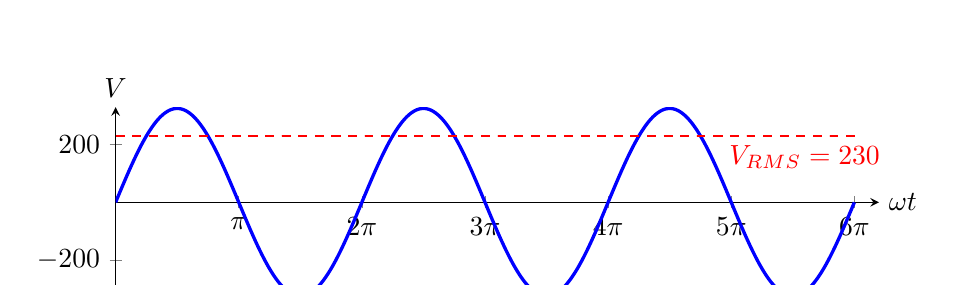
\begin{tikzpicture}
            \begin{axis}[
                    domain=0:6*pi,
                    samples=3*360,
                    xtick={0, pi, 2*pi, 3*pi, 4*pi, 5*pi, 6*pi},
                    xticklabels={\(0\), \(\pi\), \(2\pi\), \(3\pi\), \(4\pi\), \(5\pi\), \(6\pi\)},
                    width=0.93\textwidth, height=4cm,
                    ymin=-330,
                    ymax = 330,
                    xmax = 6.2*pi,
                    axis lines = center,
                    xlabel style={right},
                    ylabel style={above},
                    ylabel={$V$},
                    xlabel={$\omega t$}
                ]
                \addplot [very thick, blue] {325.269*sin(deg(x))};
                \addplot [dashed, mark=none, red]{230} node[below, pos=0.95]{$V_{RMS} = \qty{230}{\volt}$};
            \end{axis}
        \end{tikzpicture}
    }

    Source voltage

    \fbox{
        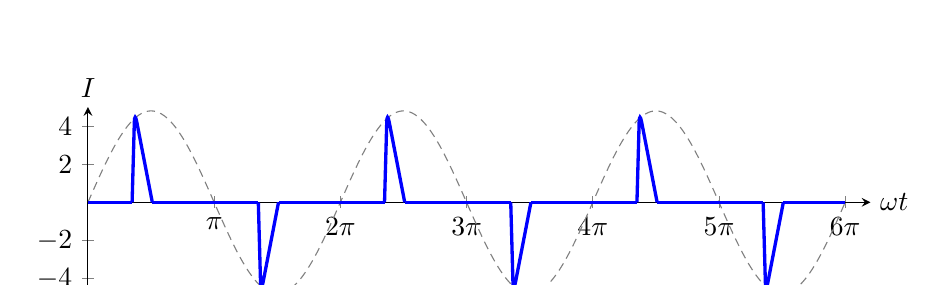
\begin{tikzpicture}
            \begin{axis}[
                    domain=0:6*pi,
                    xtick={0, pi, 2*pi, 3*pi, 4*pi, 5*pi, 6*pi},
                    xticklabels={\(0\), \(\pi\), \(2\pi\), \(3\pi\), \(4\pi\), \(5\pi\), \(6\pi\)},
                    width=0.95\textwidth, height=4cm,
                    ymin=-5,
                    ymax = 5,
                    xmax = 6.2*pi,
                    axis lines = center,
                    xlabel style={right},
                    ylabel style={above},
                    ylabel={$I$},
                    xlabel={$\omega t$}
                ]
                \addplot [densely dashed, gray, samples=3*360] {4.8*sin(deg(x))};

                \foreach \n in {0,2*pi,4*pi}
                    {
                        \addplot [very thick, blue,domain=\n:\n + 0.35*pi] {0};
                        \addplot [very thick, blue,rounded corners,samples=100] coordinates{
                                (\n +0.35*pi,0)
                                (\n +0.37*pi,4.8)
                                (\n +0.51*pi,0)
                            };
                        % \addplot [very thick, blue] coordinates{
                        %     (\n+0.51*pi,0.55)
                        %     (\n+0.51*pi,0)
                        % };
                        % \addplot [very thick, blue, domain=\n + 0.35*pi:\n + 0.51*pi]{0.55*sin(deg(x))};
                        \addplot [very thick, blue,domain=\n + 0.51*pi:\n + 1.35*pi] {0};
                        \addplot [very thick, blue,rounded corners,samples=10] coordinates{
                                (\n +1.35*pi,0)
                                (\n +1.37*pi,-4.8)
                                (\n +1.51*pi, 0)
                            };
                        % \addplot [very thick, blue] coordinates{
                        %     (\n +1.51*pi,-0.55)
                        %     (\n +1.51*pi,0)
                        % };
                        % \addplot [very thick, blue, domain=\n + 1.35*pi:\n + 1.51*pi]{0.55*sin(deg(x))};
                        \addplot [very thick, blue,domain=\n + 1.51*pi:\n + 2*pi] {0};
                    }
            \end{axis}
        \end{tikzpicture}
    }

    Source current
\end{center}

Alternatively, smoothing using an LC filter can be used, but first, the inductor value must be specified.
\begin{align*}
    \frac{\Delta V}{V_{out}} & = \frac{\sqrt{2}}{3} \left[\frac{1}{(4 \pi f)^2 L C -1}\right]                              \\
    \frac{6}{30}             & = \frac{\sqrt{2}}{3} \left[\frac{1}{(200\pi)^2 L \cdot \qty{8.4}{\milli\farad} - 1 }\right] \\
    \implies L               & = \qty{948.8}{\micro\henry}
\end{align*}

The following circuit now has an LC filtering element.
\vspace{4mm}

\begin{center}
    \begin{circuitikz}[
            american,
            % circuitikz/voltage/american,
            circuitikz/straight=true,
            full diodes,
            circuitikz/diodes/scale=0.5
        ]
        \ctikzset{quadpoles/transformer/height=2.15}
        \ctikzset{transformer L1/.style={inductors/coils=7, inductors/width=1.4}}
        \ctikzset{transformer L2/.style={inductors/coils=5, inductors/width=1}}
        % v source
        \draw (0,0) to [sV,v<=$\qty{230}{\volt_{RMS}}$] ++(0,3) -- ++(1,0)
        node[transformer, anchor=A1](T){19:2};
        \draw (T.A2) to [short] (0,0);
        % transformer output
        \draw (T.B1) -- ++(2,0) -- ++(0,-0.5) coordinate(bridge top);
        % diode bridge
        \draw (bridge top) to [D, *-*, v^=$\qty{0.7}{\volt}$] ++(1,-1) coordinate(bridge right)
        to [D, *-*, invert] ++(-1,-1) coordinate(bridge bottom)
        to [D, *-*, invert] ++(-1,1) coordinate(bridge left)
        to [D, *-*] (bridge top);
        % bridge to trans
        \draw (bridge bottom) -- ++(0,-0.5) to [short] (T.B2);
        %inductor
        \draw (bridge right) to [short] ++(1,0)
        to [L, l=$\qty{948.8}{\micro\henry}$] ++(1.5,0) coordinate(ind right);
        % capacitor
        \draw (ind right) to [short] ++(0.5,0) coordinate(cap top)
        to [C, l=$\qty{8.4}{\milli\farad}$, *-*] ++(0,-2) coordinate(cap bottom)
        to [short] ++(-5,0) -- (bridge left);
        % load
        \draw (cap top) to [short] ++(1.5,0)
        to [short, i=$\qty{5}{\ampere}$] ++(1,0)
        to [open, o-o, v=$\sim\qty{30}{\volt}$] ++(0,-2)
        -- (cap bottom);
        % voltage drops        
        \draw (T.B1) to [open, v=$\qty{34.2}{\volt}$] (T.B2);
        \draw (bridge right) ++(0.5,0) to [open, v=$\qty{32.8}{\volt}$] ++(0,-2);
    \end{circuitikz}
\end{center}

The resultant voltage waveform remains the same at the source (although the load voltage will have
reduced slightly without modifications to the windings etc.), however
the current waveform appears as follows:
\begin{center}
    \frame{\includegraphics[width=\textwidth]{1.1 lc.png}}

    Source current
\end{center}
\subsection{}


\section{DC-DC Converter Design and Specifications}
\label{sec:specification}
$   % parameters
    V_{in} = \qty{30}{\volt} \\
    V_{out} = \qty{48}{\volt} \\
    P = \qty{100}{\watt} \\
    \Delta V = \qty{100}{\milli\volt} \\
    f = \qty{25}{\kilo\hertz} \implies T = \qty{4d-5}{\second}
$

From the parameters above, the peak current can be found. The inductor needs to operate above this.
Furthermore, the capacitor needs to operate above $V_{out}$.
\begin{align*}  % current max
    I_{max} & = \frac{P}{V_{out}}                                    \\
            & = \frac{\qty{100}{\watt}}{\qty{48}{\volt}}             \\
            & = \qty[parse-numbers=false]{2.08\overline{3}}{\ampere}
\end{align*}
Using this, the duty cycle can be found.
\begin{align*}  % duty cycle
    \rho & = 1 - \frac{V_{out}}{V_{in}}                  \\
         & = 1 - \frac{\qty{30}{\volt}}{\qty{48}{\volt}} \\
         & = \frac{3}{8}
\end{align*}
Finally, the capacitor and inductor values can be calculated.
\begin{align*}  % capacitor
    C_{out} & = \frac{I_{max}\rho}{f \cdot \Delta V}                                                                                                  \\
            & = \frac{ \qty[parse-numbers=false]{2.08\overline{3}}{\ampere} \cdot \frac{3}{8} }{ \qty{25}{\kilo\hertz} \cdot \qty{100}{\milli\volt} } \\
            & = \qty{312}{\micro\farad}
    \\ \\
    L       & = \frac{V_{in} \rho T}{2 \cdot I_{max}}                                                                                                 \\
            & = \frac{ \qty{30}{\volt} \cdot \frac{3}{8} \cdot \qty{4d-5}{\second} }{2 \cdot \qty[parse-numbers=false]{2.08\overline{3}}{\ampere} }   \\
            & = \qty{104}{\micro\henry}
\end{align*}

The found capacitor and inductor values are the minimum, therefore the next highest value
of the units available need to be used. The \qty{150}{\micro\henry} (rated \qty{6.5}{\ampere})
inductor and \qty{330}{\micro\farad} (rated \qty{63}{\volt}) capacitor are chosen.


\section{Boost Convertor Experiment Report}

\subsection{Abstract}

The purpose of this laboratory was to design a DC/DC \qty{30}{\volt}-\qty{48}{\volt} boost converter and experimentally test its performance.
The boost convertor designed was subjected to up to a \qty{75}{\watt} load in \qty{25}{\watt} increments, with measurements taken of various parameters,
including output voltage, inductor current, and duty ratios of the converter switching transistor. 
The circuit was not tested to the designed conditions precisely, and therefore does not perform 
exactly to specification. For most areas except ripple voltage, the circuit parameters are within 
reasonable expection.

Furthermore, different switching control systems were used to compare the 
performance of the circuit under changing conditions. The results show that the circuit 
performance can be improved for specific metrics, however some trade-offs need to be made. Open-loop control
is the simplest to implement and no further power draining circuitry, however suffers from limited 
flexibility to changing loads. Proportional control introduces extra load on the circuit, but does not
manage to make power efficiency improvements to counteract this. It did have the quickest response time.
 Proportional and integral control showed the best efficiency,however suffered the greatest
  rise time and may not be suitable in applications where response time is vital. 

\subsection{Introduction}
\subsubsection{Aims}
This report will detail the process of experimentally testing the performance of the boost converter,
parameters for which specified in \hyperref[sec:specification]{Section 2}.
The experiment additionally tests the converter performance under different control systems: open-loop control,
proportional control, and finally proportional and integral control.

The experiment will be used to compare theoretical ideal performance to observed real performance under different conditions.

\subsubsection{Theory}
A boost converter ensures that the output voltage is higher than the input voltage. It does this by leveraging an inductor's
tendency to oppose changes in current by adjusting its voltage.

The following diagram demonstrates a simple boost converter circuit, as will be used in this experiment.
\begin{center}
    \begin{circuitikz}[
            american,
            % circuitikz/voltage/american,
            circuitikz/straight=true,
            full diodes,
            circuitikz/diodes/scale=0.5,
        ]
        \draw (0,0) to [short, o-*] ++(2,0) coordinate(ind start)   %inductor
        to [L, l=$L$] ++(3,0) coordinate(ind end)
        to [D, *-*] ++(2,0) coordinate(diode end)
        to [short, *-o] ++(2,0) coordinate(end);
        \draw (ind end) to [short] ++(0,-2) node[nigfete, bodydiode, tr circle=true](fet){} %fet
        (fet.G) node[anchor=east]{$V_{GS}$}
        (fet.D) node[anchor=south east]{$V_{DS}$}
        (fet.S) to [short] ++(0,-1.2);
        \draw (diode end) to [C,l=$C_{out}$, *-*] ++(0,-4) coordinate(cap bottom); % cap out
        \draw (end) to [open, v=$V_{out}$] ++(0,-4)
        to [short, o-*] ++(-4,0)
        to [R, *-*, l=$R$] ++(0,-2)
        to [short, *-*] ++(-3,0)
        to [short, *-o] ++(-2,0);
        \draw (ind start) to [short] ++(0,-2)
        to [C, l=$C_{in}$] ++(0,-2) to [short] ++(0,-2);
        \draw (0,0) to [open, v=$V_{in}$] ++(0,-6);
    \end{circuitikz}
\end{center}

The converter circuit operates in two states depending on whether the MOSFET switch is `open' (not
conducting) or `closed' (conducting).

\paragraph{Open}
Current flows to the diode and capacitor, resulting in higher overall circuit impedance. The inductor compensates
by developing a voltage in series with the source in order to maintain current from the `closed' stage.
This results in a greater voltage at the output.
\paragraph{Closed}
Current flows throught the MOSFET as the path of least resistance, effectively closing the circuit
off from the diode onwards. The inductor charges its magnetic field during this stage. The output capacitor $C_{out}$ maintains
the voltage to the output during this stage, as it was charged to the voltage of the parallel output.
The diode prevents backflow from the capacitor.

\paragraph{Continuous mode}
Continuous mode for a boost converter means the inductor current is continous - in other words, it never drops to 0 or becomes discontinuous.
Discontinous conduction can occur if the current ripple is too large (due to insufficient load) or the MOSFET is not
switched quickly enough ($V_{GS}$ is pulsed too slowly), allowing the inductor to discharge completely.

\paragraph{Additional components}
The circuit specified uses two additional components that are not fundamental to an ideal boost converter circuit.
Resistor $R$ manages large current discharge through the MOSFET during the `closed' stage. Capacitor $C_{out}$ smooths the input
as the DC signal is not ideally flat.

\paragraph{Control systems}
The experiment will be performed with three control systems: open-loop, proportional, and proportional and integral control. Open-loop control requires the response of the circuit to be adjusted externally.
While the simplest to implement, it requires external input to adjust for any changes in the load. Closed-loop systems, on the other hand, can respond to changing conditions
automatically with no external input required. However, reduced steady-state error may come at the cost of greater response time, especially
where integral controllers are used. With no differential controller, overshoot is also likely to increase. Many of these drawbacks can be minimised with suitable parameter choices,
however this requires complex analysis of the system and its responses, and would likely prove to become more complex than the boost converter circuit itself.

\subsection{Method}
\subsubsection{Equipment}
The experiment requires a number of components in order to test the design. The design portion of this experiment involves
selecting an inductor and capacitor from an available range.

In addition to these two components, the following equipment is also required:
\begin{itemize}
    \item ES3E0 experimental test board - comes with:
          \begin{itemize}
              \item IRFI14110G MOSFET
              \item UF5401 diode
              \item LM3524 PWM controller
          \end{itemize}
    \item \qty{36}{\volt} capable DC power supply
    \item Oscilloscope
    \item \qty{100}{\watt} load bank with \qty{25}{\watt} increments - caution: may get hot with
          continuous load; use for minimum time necessary for measurements
    \item Voltmeter
    \item Ammeter
\end{itemize}


\subsubsection{Method}
\paragraph{Setup}
\begin{enumerate}
    \item Connect the power supply to the experimental test board \qty{0}{\volt} and VIN terminals
    \item Set the output voltage of the power supply to \qty{30}{\volt}
    \item Set the current limit to \qty{6}{\A}
    \item Ensure VOUT SET is at minimum (turned fully anti-clockwise)
    \item Fit the chosen specified capacitor and inductor into the board. Also include an input capcitor as part of the circuit (can be of any appropriate size - \qty{1000}{\uF} suggested)
    \item Connect the load bank to the boost converter output (VOUT), including an ammeter in series and a voltmeter in parallel
    \item Ensure the load bank is switched off (\qty{0}{\percent})
    \item With everything set up, enable the power supply
\end{enumerate}

\paragraph{Open-loop system test}
\subparagraph{Purpose}
The boost converter is operated in open-loop mode. The VOUT SET potentiometer on the experimental board
controls the duty cycle of the MOSFET, thereby manually setting the output voltage of the converter.

The steady-state power losses and output voltage ripples will be measured.

There are two experiments performed to test the open-loop system parameters: steady-state and transient.
The steady-state test observes how the converter works under typical use. The transient test observes
the converter when it is first powered on with no load.

\subparagraph{Steady-state}
Switch SW1 (LOOP CONTROL) to OPEN and SW4 (STEP INPUT) to OFF. Set the load bank to \qty{50}{\percent} by switching on two switches.
Set the output voltage to \qty{48}{\volt} using the VOUT SET potentiometer. This can be done using the rotating
the potentiometer clockwise until the multimeter across the output reads \qty{48}{\volt}.\\
Record:
\begin{enumerate}
    \item Inductor current
          \begin{itemize}
              \item Maximum
              \item Minimum
              \item Period
          \end{itemize}
    \item Output voltage ripple
          \begin{itemize}
              \item Maximum
              \item Minimum
              \item Period
          \end{itemize}
    \item Duty ratio
    \item Switching frequency
    \item Voltages V\textsubscript{GS} and V\textsubscript{DS}
    \item Input and output voltages and currents
\end{enumerate}
The power supplied and provided, and subsequently the overall efficiency can then be calculated.

\subparagraph{Transient}
Set the load bank to \qty{25}{\percent} by switching on one switch and set VOUT SET to minimum
by rotating fully anti-clockwise.
Switch STEP INPUT from OFF to STEP 1 to introduce a step input signal.
The oscilloscope will need to be set up to record \qty{35}{\volt} rising edge transients. \\
Record:
\begin{enumerate}
    \item Initial voltage
    \item Final voltage
    \item Start time
    \item End time
\end{enumerate}
Repeat this experiment with the load bank set to \qty{50}{\percent} by switching on an additional switch.

\paragraph{Closed-loop system test}
\subparagraph{Purpose}
Manually setting the duty cycle suffers from not only limited accuracy but also difficulty maintaining a setpoint where the load varies.
Closed-loop system control uses feedback to adjust the duty cycle in order to account for flunctuating load, thereby maintaining the
desired setpoint. This can be achieved by using a proportional and integral (PI) controller.

Two tests will be defined - one with proportional control only, and a second with proportional and integral control.
\subparagraph{Proportional control}
Set switch SW1 to PI CTRL, SW2 to Integrator OUT, SW4 to Step input OFF. Ensure the VOUT SET potentiometer is set to minimum (turned
fully anti-clockwise). Set load to \qty{25}{\percent}. Switch Step Input to STEP 1. Adjust the proportional gain potentiometer ($K_P$)
to give an output of \qty{35}{\V}. Toggle the Step Input switch to measure both transient and steady-state parameters.\\
Record:
\begin{itemize}
    \item Transients
          \begin{enumerate}
              \item Initial voltage
              \item Final voltage
              \item Start time
              \item End time
          \end{enumerate}
    \item Ripple
          \begin{enumerate}
              \item Maximum voltage
              \item Minimum voltage
              \item Period
          \end{enumerate}
    \item Proportional controller output
    \item Duty ratio, especially during transient period
    \item Input and output voltages and currents
\end{itemize}

Repeat the experiment with the load set to \qty{50}{\percent}. Additionally, change the reference voltage to \qty{40}{\volt} by switching
Step Input from STEP 1 to STEP 2, holding the position to take readings.

\subparagraph{Proportional and integral control}
Set switch SW2 to integrator IN and SW4 STEP INPUT to OFF. Wnsure VOUT SET is at minimum (turned fully anti-clockwise).
Reset proportional (K\textsubscript{P}) and integrator (K\textsubscript{I}) potentiometers to centre. Switch integral capacitor SW3 to \qty{47}{\nF}.
Set load to \qty{50}{\percent} and STEP INPUT from OFF to STEP 1.\\
Record:
\begin{itemize}
    \item Transients
          \begin{enumerate}
              \item Initial voltage
              \item Final voltage
              \item Start time
              \item End time
          \end{enumerate}
    \item Ripple
          \begin{enumerate}
              \item Maximum voltage
              \item Minimum voltage
              \item Period
          \end{enumerate}
    \item Proportional and integral controller output
    \item Duty ratio, especially during transient period
    \item Input and output voltages and currents
\end{itemize}

Repeat the experiment with the load set to \qty{75}{\percent}.
% \paragraph{Steady-state}
\clearpage
\subsection{Results}
\subsubsection{Open-loop system tests}
\begin{table}[H]
    \centering
    \caption{\textbf{Open-loop steady-state inductor current (measured at \qty{50}{\milli\volt\per\ampere})}}
    \begin{tabularx}{\columnwidth}{|X|X|X|X|X|X|X|}
        \hline
        Maximum current & Minimum current & Peak-to-peak ripple current & Average current & Period           & Frequency        \\
        \hline
        \qty{3.58}{\A}  & \qty{0.22}{\A}  & \qty{3.36}{\A}              & \qty{1.9}{\A}   & \qty{42.40}{\us} & \qty{23.6}{\kHz} \\
        \hline
    \end{tabularx}
    \label{table:inductor}
\end{table}
\begin{figure}[H]
    \includegraphics[width=0.7\textwidth]{inductor current.png}
    \centering
    \caption{Inductor current (measured at \qty{50}{\milli\volt\per\ampere})}
\end{figure}

\begin{table}[H]
    \centering
    \caption{\textbf{Open-loop steady-state ripple voltage}}
    \begin{tabularx}{\columnwidth}{|X|X|X|X|X|X|}
        \hline
        Maximum voltage  & Minimum voltage   & Peak-to-peak ripple voltage & Period           & Frequency        \\
        \hline
        \qty{254.0}{\mV} & \qty{-274.0}{\mV} & \qty{528}{\mV}              & \qty{42.40}{\us} & \qty{23.6}{\kHz} \\
        \hline
    \end{tabularx}
    \label{table:olssrv}
\end{table}
\begin{figure}[H]
    \includegraphics[width=0.7\textwidth]{output voltage 1.png}
    \centering
    \caption{Ripple voltage}
\end{figure}


\begin{table}[H]
    \centering
    \caption{\textbf{Open-loop steady-state switching signals}}
    \begin{tabularx}{\columnwidth}{|X|X|X|X|X|}
        \hline
        Duty ratio  & Frequency        & V\textsubscript{GS} voltage & V\textsubscript{DS} voltage \\
        \hline
        \num{0.575} & \qty{23.6}{\kHz} & \qty{22.0}{\V}              & \qty{49.6}{\V}              \\
        \hline
    \end{tabularx}
\end{table}
\begin{figure}[H]
    \begin{subfigure}{0.5\textwidth}
        \includegraphics[width=\textwidth]{mosfet duty cycle.png}
        \caption{Duty cycle measurement}
    \end{subfigure}
    \hfill
    \begin{subfigure}{0.5\textwidth}
        \includegraphics[width=\textwidth]{mosfet terminal.png}
        \caption{Terminal voltages \textcolor{Magenta1}{V\textsubscript{GS}} and \textcolor{green}{V\textsubscript{DS}}}
    \end{subfigure}
    \caption{Switching signals}
\end{figure}

\begin{table}[H]
    \centering
    \caption{\textbf{Open-loop steady-state efficiency}}
    \begin{tabularx}{\columnwidth}{|X|X|X|X|X|X|X|}
        \hline
        Input current       & Output current      & Input voltage & Output voltage & Input power       & Output power      & Efficiency           \\
        \hline
        \qty{1.91}{\ampere} & \qty{1.02}{\ampere} & \qty{30}{\V}  & \qty{48}{\V}   & \qty{57.3}{\watt} & \qty{49.0}{\watt} & \qty{85.5}{\percent} \\
        \hline
    \end{tabularx}
    \label{table:olsse}
\end{table}

% \paragraph{Transient}
\begin{table}[H]
    \centering
    \caption{\textbf{Open-loop transient parameters}}
    \begin{tabularx}{\columnwidth}{|X|X|X|X|X|}
        \hline
        Initial voltage & Final voltage     & Start time       & End time         & Rise time       \\
        \hline
        \multicolumn{5}{|c|}{\qty{25}{\percent} load}                                               \\
        \hline
        \qty{30}{\volt} & \qty{41.8}{\volt} & \qty{-3.66}{\ms} & \qty{15.24}{\ms} & \qty{18.9}{\ms} \\
        \hline
        \multicolumn{5}{|c|}{\qty{50}{\percent} load}                                               \\
        \hline
        \qty{30}{\volt} & \qty{37.6}{\volt} & \qty{-3.06}{\ms} & \qty{1.34}{\ms}  & \qty{4.4}{\ms}  \\
        \hline
    \end{tabularx}
    \label{table:oltrans}
\end{table}
\begin{figure}[H]
    \begin{subfigure}{0.5\textwidth}
        \includegraphics[width=\textwidth]{transient load 25.png}
        \caption{\qty{25}{\percent} load}
    \end{subfigure}
    \hfill
    \begin{subfigure}{0.5\textwidth}
        \includegraphics[width=\textwidth]{transient load 50.png}
        \caption{\qty{50}{\percent} load}
    \end{subfigure}
    \caption{Transient parameters}
\end{figure}



\subsubsection{Closed-loop system test}
% \paragraph{Proportional control}
\begin{table}[H]
    \centering
    \caption{\textbf{Proportional control transient parameters (\qty{25}{\percent} load)}}
    \begin{tabularx}{\columnwidth}{|X|X|X|X|X|}
        \hline
        Initial voltage   & Final voltage     & Start time       & End time         & Rise time      \\
        \hline
        \qty{28.6}{\volt} & \qty{34.8}{\volt} & \qty{-2.06}{\ms} & \qty{440.0}{\us} & \qty{2.5}{\ms} \\
        \hline
    \end{tabularx}
\end{table}
\begin{figure}[H]
    \begin{subfigure}{0.5\textwidth}
        \includegraphics[width=\textwidth]{proportional transient.png}
        \caption{Transient capture}
    \end{subfigure}
    \hfill
    \begin{subfigure}{0.5\textwidth}
        \includegraphics[width=\textwidth]{proportional controller.png}
        \caption{Proportional controller response}
    \end{subfigure}
    \caption{Transient parameters (\qty{25}{\percent} load)}
    \label{fig:controllerresponse}
\end{figure}

\begin{table}[H]
    \centering
    \caption{\textbf{Proportional control ripple voltage (\qty{25}{\percent} load)}}
    \begin{tabularx}{\columnwidth}{|X|X|X|X|X|}
        \hline
        Maximum voltage        & Minimum voltage        & Peak-to-peak ripple & Period          & Frequency        \\
        \hline
        \qty{180}{\milli\volt} & \qty{-48}{\milli\volt} & \qty{228.0}{\mV}    & \qty{42.4}{\us} & \qty{23.6}{\kHz} \\
        \hline
    \end{tabularx}
\end{table}
\begin{figure}[H]
    \centering
    \includegraphics[width=0.7\textwidth]{tek00005.png}
    \caption{Ripple voltage (\qty{25}{\percent} load)}
\end{figure}

\begin{table}[H]
    \centering
    \caption{\textbf{Proportional control efficiency (\qty{25}{\percent} load)}}
    \begin{tabularx}{\columnwidth}{|X|X|X|X|X|X|X|}
        \hline
        Input current        & Output current       & Input voltage  & Output voltage & Input power        & Output power       & Efficiency           \\
        \hline
        \qty{0.564}{\ampere} & \qty{0.384}{\ampere} & \qty{30.0}{\V} & \qty{35.0}{\V} & \qty{16.92}{\watt} & \qty{13.44}{\watt} & \qty{79.4}{\percent} \\
        \hline
    \end{tabularx}
\end{table}

\begin{table}[H]
    \centering
    \caption{\textbf{Proportional control transient parameters (\qty{50}{\percent} load)}}
    \begin{tabularx}{\columnwidth}{|X|X|X|X|X|}
        \hline
        Initial voltage   & Final voltage   & Start time      & End time       & Rise time     \\
        \hline
        \qty{33.8}{\volt} & \qty{40}{\volt} & \qty{-5.4}{\ms} & \qty{4.6}{\us} & \qty{10}{\ms} \\
        \hline
    \end{tabularx}
\end{table}
\begin{figure}[H]
    \begin{subfigure}{0.5\textwidth}
        \includegraphics[width=\textwidth]{tek00007.png}
        \caption{Transient capture}
    \end{subfigure}
    \hfill
    \begin{subfigure}{0.5\textwidth}
        \includegraphics[width=\textwidth]{tek00008.png}
        \caption{P controller response}
        \label{fig:prop50control}
    \end{subfigure}
    \caption{Transient parameters (\qty{50}{\percent} load)}

\end{figure}

\begin{table}[H]
    \centering
    \caption{\textbf{Proportional control ripple voltage (\qty{50}{\percent} load)}}
    \begin{tabularx}{\columnwidth}{|X|X|X|X|X|}
        \hline
        Maximum voltage        & Minimum voltage         & Peak-to-peak ripple & Period          & Frequency        \\
        \hline
        \qty{218}{\milli\volt} & \qty{-194}{\milli\volt} & \qty{412.0}{\mV}    & \qty{43.0}{\us} & \qty{23.3}{\kHz} \\
        \hline
    \end{tabularx}
    \label{table:prop50ripple}
\end{table}

\begin{figure}[H]
    \begin{subfigure}{0.5\textwidth}
        \includegraphics[width=\textwidth]{tek00009.png}
        \caption{Ripple voltage (\qty{50}{\percent} load)}
    \end{subfigure}
    \hfill
    \begin{subfigure}{0.5\textwidth}
        \includegraphics[width=\textwidth]{tek00012.png}
        \caption{Duty cycle}
        \label{fig:prop50dutycycle}
    \end{subfigure}
    \caption{Output captures}
\end{figure}

\begin{table}[H]
    \centering
    \caption{\textbf{Proportional control efficiency (\qty{50}{\percent} load)}}
    \begin{tabularx}{\columnwidth}{|X|X|X|X|X|X|X|}
        \hline
        Input current        & Output current       & Input voltage  & Output voltage & Input power        & Output power       & Efficiency           \\
        \hline
        \qty{1.344}{\ampere} & \qty{0.857}{\ampere} & \qty{30.0}{\V} & \qty{40.2}{\V} & \qty{40.32}{\watt} & \qty{34.45}{\watt} & \qty{85.4}{\percent} \\
        \hline
    \end{tabularx}
\end{table}

\clearpage
\begin{table}[H]
    \centering
    \caption{\textbf{Proportional and integral control transient parameters (\qty{50}{\percent} load)}}
    \begin{tabularx}{\columnwidth}{|X|X|X|X|X|}
        \hline
        Initial voltage   & Final voltage     & Start time       & End time        & Rise time        \\
        \hline
        \qty{28.8}{\volt} & \qty{34.8}{\volt} & \qty{-51.4}{\ms} & \qty{55.4}{\us} & \qty{106.8}{\ms} \\
        \hline
    \end{tabularx}
\end{table}
\begin{figure}[H]
    \begin{subfigure}{0.5\textwidth}
        \includegraphics[width=\textwidth]{tek00013.png}
        \caption{Transient capture}
        \label{fig:pi50trans}
    \end{subfigure}
    \hfill
    \begin{subfigure}{0.5\textwidth}
        \includegraphics[width=\textwidth]{tek00014.png}
        \caption{PI controller response}
        \label{fig:pi50controller}
    \end{subfigure}
    \caption{Transient parameters (\qty{50}{\percent} load)}
\end{figure}

\begin{table}[H]
    \centering
    \caption{\textbf{Proportional and integral control ripple voltage (\qty{50}{\percent} load)}}
    \begin{tabularx}{\columnwidth}{|X|X|X|X|X|}
        \hline
        Maximum voltage        & Minimum voltage        & Peak-to-peak ripple & Period          & Frequency        \\
        \hline
        \qty{710}{\milli\volt} & \qty{380}{\milli\volt} & \qty{330}{\mV}      & \qty{42.4}{\us} & \qty{23.6}{\kHz} \\
        \hline
    \end{tabularx}
    \label{table:pi50ripple}
\end{table}

\begin{figure}[H]
    \centering
    \includegraphics[width=0.7\textwidth]{tek00017.png}
    \caption{Duty cycle}
\end{figure}

\begin{table}[H]
    \centering
    \caption{\textbf{Proportional and integral control efficiency (\qty{50}{\percent} load)}}
    \begin{tabularx}{\columnwidth}{|X|X|X|X|X|X|X|}
        \hline
        Input current        & Output current       & Input voltage  & Output voltage  & Input power        & Output power       & Efficiency           \\
        \hline
        \qty{1.045}{\ampere} & \qty{0.755}{\ampere} & \qty{30.0}{\V} & \qty{35.41}{\V} & \qty{31.35}{\watt} & \qty{26.73}{\watt} & \qty{85.3}{\percent} \\
        \hline
    \end{tabularx}
\end{table}

\begin{table}[H]
    \centering
    \caption{\textbf{Proportional and integral control transient parameters (\qty{75}{\percent} load)}}
    \begin{tabularx}{\columnwidth}{|X|X|X|X|X|}
        \hline
        Initial voltage   & Final voltage     & Start time      & End time       & Rise time      \\
        \hline
        \qty{28.4}{\volt} & \qty{36.0}{\volt} & \qty{-266}{\ms} & \qty{-80}{\us} & \qty{186}{\ms} \\
        \hline
    \end{tabularx}
\end{table}
\begin{figure}[H]
    \begin{subfigure}{0.5\textwidth}
        \includegraphics[width=\textwidth]{tek00020.png}
        \caption{Transient capture}
    \end{subfigure}
    \hfill
    \begin{subfigure}{0.5\textwidth}
        \includegraphics[width=\textwidth]{tek00021.png}
        \caption{PI controller response}
    \end{subfigure}
    \caption{Transient parameters (\qty{75}{\percent} load)}
\end{figure}

\begin{table}[H]
    \centering
    \caption{\textbf{Proportional and integral control ripple voltage (\qty{75}{\percent} load)}}
    \begin{tabularx}{\columnwidth}{|X|X|X|X|X|}
        \hline
        Maximum voltage        & Minimum voltage        & Peak-to-peak ripple & Period          & Frequency        \\
        \hline
        \qty{770}{\milli\volt} & \qty{440}{\milli\volt} & \qty{330}{\mV}      & \qty{41.6}{\us} & \qty{24.0}{\kHz} \\
        \hline
    \end{tabularx}
\end{table}

\begin{figure}[H]
    \begin{subfigure}{0.5\textwidth}
        \includegraphics[width=\textwidth]{tek00023.png}
        \caption{Ripple voltage (\qty{75}{\percent} load)}
    \end{subfigure}
    \hfill
    \begin{subfigure}{0.5\textwidth}
        \includegraphics[width=\textwidth]{tek00026.png}
        \caption{Duty cycle}
    \end{subfigure}
    \caption{Output captures}
\end{figure}

\begin{table}[H]
    \centering
    \caption{\textbf{Proportional and integral control efficiency (\qty{75}{\percent} load)}}
    \begin{tabularx}{\columnwidth}{|X|X|X|X|X|X|X|}
        \hline
        Input current        & Output current       & Input voltage  & Output voltage  & Input power        & Output power       & Efficiency           \\
        \hline
        \qty{1.509}{\ampere} & \qty{1.119}{\ampere} & \qty{30.0}{\V} & \qty{35.41}{\V} & \qty{45.27}{\watt} & \qty{39.62}{\watt} & \qty{87.5}{\percent} \\
        \hline
    \end{tabularx}
\end{table}
\clearpage

\subsection{Analysis}
\paragraph{Open-loop system}
\subparagraph{Steady-state}
The first tests involve an open-loop control system.
Here (\autoref{table:inductor}), the inductor
parameters were observed. The inductor is operating comfortably below
its maximum rated current. Conduction is on the threshold of dicontinuity.\\
The steady-state peak-to-peak ripple voltage voltage (\autoref{table:olssrv})
reaches \qty{528}{\mV} which is somewhat large, however ultimately \qty{1}{\percent} of the output.\\
The frequency of both signals and transistor switching align, which is expected.
The $V_{DS}$ voltage is larger than the output voltage which hints to losses occuring
within the circuit.\\
Efficiency appears at \qty{85.5}{\percent}, which is quite good. Power draw is fairly large, but not
out of expectation due to the large voltage requirements.
\subparagraph{Transient}
The transient parameters in \autoref{table:oltrans} show different responses to
increased load. The final voltage is lower than expected, likely due to an error in the
experimental procedure where the duty ratio was set with no load. Qualitatively, the output
voltage decreases with a greater load, as does the rise time (by a factor of 7.5).

\paragraph{Proportional control}
\subparagraph{\qty{25}{\percent} load}
The initial voltage is slightly below \qty{30}{\volt}.
The output voltage was set at \qty{35}{\volt} which is somewhat smaller which may have led to
a quicker rise time of the circuit (\qty{2.5}{\ms}).
\autoref{fig:controllerresponse} shows the proportional controller begin pulsing rapidly
and continuously once the converter is enabled. The peak-to-peak ripple has also reduced to
\qty{228}{\mV}, suggesting a smoother circuit. The frequency has as yet remained the same.\\
Due to the smaller output, the current draw requirements are also smaller, with almost a quarter
the current draw of the open-loop circuit. The efficiency has decreased, which suggests that the
controller introduces some losses on the circuit.
\subparagraph{\qty{50}{\percent} load}
The initial voltage is not \qty{30}{\volt} due to the experiment being performed with an
increase to \qty{50}{\percent} from \qty{25}{\percent}, rather than from \qty{0}{\percent}.
This may have reduced the rise time. This is further evidenced by the controller in \autoref{fig:prop50control}
operating in the `initial' region. After the load is increased, the controller responds by
pulsing more frequently.\\
The frequency appears to have decreased, however this may be within measurement error
as, while the period for the ripple voltage in \autoref{table:prop50ripple} has increased,
the period in \autoref{fig:prop50dutycycle} appears the same as in previous experiments.\\
Efficiency has increased by six percentage points, which indicates better power management on either
higher loads or higher output voltages.

\paragraph{Proportional and integral control}
\subparagraph{\qty{50}{\percent} load}
The initial voltage is slightly below \qty{30}{\volt} at \qty{28.8}{\volt}. The final voltage is
well met, with a deficiency of \qty{0.2}{\volt} from the specified \qty{35}{\volt}. The rise time
is an order of magnitude greater than in previous tests. The ripple voltage in \autoref{fig:pi50trans}
appears greater than in previous tests, however this is likely due to the use of a different timescale.
Similarly, the PI controller response appears to have a larger wavelength. \autoref{fig:pi50controller}
does not demonstrate the change in controller response across the rise due to experimental error in
the transient capture.\\
As mentioned, the ripple appears greater than it actually is. As per \autoref{table:pi50ripple}, the
peak-to-peak ripple is \qty{330}{\mV}, which is smaller than the ripple with proportional control
only (\qty{412}{\mV}). The frequency \qty{23.6}{\kHz} again. \\
Efficiency sits at \qty{85.3}{\percent}, which indicates similar performance to the proportional
controller.
\subparagraph{\qty{75}{\percent} load}
Initial voltage is slightly below \qty{30}{\volt}, which is similar to the \qty{50}{\percent} load.
The final voltage has risen by \qty{1}{\volt} above the specified. Rise time has also increased
by almost double the previous.\\
Ripple voltage has decreased, which may explain the increase in frequency, however it is possible
the latter falls within the margin for error as in proportional control ripple
(\autoref{table:prop50ripple}). \\
This setup indicates the greatest efficiency yet, at \qty{87.5}{\percent}.

\subsection{Discussion}

The designed parameters were built around predicted use case values - for example, \qty{100}{\watt} load.
Furthermore, the design called for specific, non-standard values that could not be met in implementation.
This is the first of perhaps many reasons why differences exist between the designed values and the
observed results with real components. \\
One of the first assumptions was the peak current, which can more accurately be referred to as the average
current. The observed values (\qty{1.9}{\A}) was close to the calculated value (\qty{2.1}{\A}), however
this was at no load. Testing was not performed with a full \qty{100}{\watt} load, but the subsequent
experiments suggest that the current would be in this region.\\
While there is consistency here, differences begin to emerge when comparing the duty cycle and frequency
of the converter. The frequency across tests was reasonbly consistent but slightly lower than expected
by calculation. The duty cycle, on the other hand, appeared to be 0.575 rather than the expected 0.375.
The peak-to-peak ripple was also very far out of proportion (over five times as much), however this
reduced once greater loads were introduced. The ripple itself may be unsuitable for some applications as 
it over $~\qty{0.5}{\volt}$, which may be too large a variation. For equipment running at \qty{48}{\volt}
however, this is unlikely (but not a factor to ignore).\\
Some of these differences may be accounted for by the unideal performance of components in experimentation.
The theoretical calculations do not take into account losses in operation, however this is reflected in
the observed efficiency of the system at \qty{85.5}{\percent}. Overall, this efficiency is quite good,
however it may be possible to improve upon this with components that are more energy efficient. As it
stands, the circuit lost almost \qty{10}{\watt} which is significant enough that it cannot be ignored.
It is not recommended to use this circuit without any passive cooling at a minimum, and especially not in
and enclosed or compact space without mitigation for the power losses of the converter. The greatest losses
likely occured in the MOSFET due to high-frequency switching, and the resistor due to current handling.

The introduction of proportional control appears to have reduced the ripple and rise time.
 However, this came at the cost of decreased efficiency, likely 
due to greater power dissipation in the control system circuit. The reduced ripple is within expectations,
as the proportional gain should allow the circuit to respond to the ripple and conpensate. Usually,
the response takes some time, so it is surprising to see the rise time so low and the frequency remain 
the same. These findings were reflected in the \qty{50}{\watt} test. Direct comparisons are difficult 
given different output voltages and loads per test, both of which likely impact factors such as 
the peak-to-peak ripple.

The further addition of integral gain allowed noticeable improvements to the ripple voltage and 
efficiency. This occurs despite the extra load on the entire circuit with the inclusion of 
proportional and integral gain circuitry. This rise time was significantly affected adversely, however,
and is noticeably slower to switch on to the rated voltage than any other circuit. 

A few general trends could also be noticed. Rise times appeared to improve across increased loads
with all else the same. Efficiency also seemed to improve with greater output voltages. This may 
be due to the circuit loading parameters approaching those of the design. Additionally, 
frequency changes between load changes for both closed-loop controllers can be observed. 
This may fall within measurement error, however it may also be a result of the controller adapting 
the frequency to account for the increased load.

\bibliographystyle{ieeetr}
\bibliography{refs}

\end{document}